\documentclass[../main.tex]{subfiles}
\begin{document}

\section{Research Design}
This study adopts a mixed-method approach that integrates automated text analysis using a large language model (LLM) with traditional manual evaluation methods. The feasibility study is structured to assess the LLM's ability to evaluate administrative acts by comparing its outputs against those generated by human experts. The overall framework comprises data collection, checklist integration, automated querying, and performance benchmarking. 

To structure the automation process and facilitate independent testing, we conceptualized the core LLM-driven tasks as two distinct functional components, referred to here in a simplified sense as "agents". Each agent is designed to perform a single, specific action within the overall administrative control workflow. This separation allowed for a focused evaluation of the LLM's effectiveness in executing each sub-task individually.

The first agent is responsible for checklist selection. Its function is to analyze the content of an administrative act ("determina") and identify the most appropriate checklist from the predefined set, based on the descriptions and criteria embedded within each checklist's JSON definition. The second agent handles the checklist completion task. Once a checklist is selected (either manually for testing or by the first agent), this second agent systematically processes each point, querying the LLM to evaluate the determination against the specific instruction and criterion of that point, ultimately providing a compliance assessment (e.g., "SI", "NO", "NON PERTINENTE").

This modular design, while simplifying the initial feasibility study and enabling targeted performance analysis, represents an intermediate step. The intention for a future, fully integrated system is to combine these functionalities into a single, more sophisticated agent. This unified agent would autonomously perform the entire sequence: reading and understanding the administrative act, selecting the correct checklist, and then proceeding to complete the evaluation point by point, thereby fully automating the core assessment process.

\section{Data Collection Process}
Municipal documents, specifically determinations (or “determina”) available on the public bulletin (or "albo pretorio"), form the primary data source. For each document, the following steps are undertaken:

\begin{itemize}
    \item \textbf{Document Acquisition}: Download PDF files of relevant determinations.
    \item \textbf{Text Extraction}: Convert each PDF into plain text using Python-based tools, ensuring the content is accessible for further processing.
    \item \textbf{Checklist Selection}: Use a CSV file that maps the document names to their associated checklists. ( This step was done by an actual
\end{itemize}

\section{Checklists Integration}
To standardize the evaluation process, a series of checklists was compiled based on the administrative control requirements used by public administration entities. These checklists were transformed into a JSON format, allowing the division of each checklist into individual questions. Each checklist point includes specific instructions that guide the evaluation of the act in question. In the \hyperref[appendix:json_template]{Appendix} there is the template for the JSON that is used in this study (see Appendix \ref{appendix:json_template}).

\section{LLMs Usage}
The LLMs are central to this study. Its role is to analyze the text extracted from municipal determinations and respond to each point of the checklist. The process involves:

\begin{itemize}
    \item \textbf{Prompt Design and Configuration:}
    
 A structured prompt template was created to guide the LLM. The template includes:
    \begin{itemize}
        \item Instructions to the model as an expert in administrative law.
        \item A clear layout where each checklist point is presented as a question.
        \item A predefined answer format (e.g., SI/NO/NON PERTINENTE with a brief explanation if needed).
    \end{itemize}
    \item \textbf{Extraction and Analysis Process:}
    
 The LLM is queried for each checklist point using the custom prompt. The responses, initially in long text form, are processed using regular expressions to extract the essential output: namely, a categorical answer (SI, NO, NON PERTINENTE) and a concise explanation when necessary. A Python script orchestrates this process and aggregates the results into a CSV file.
    \item \textbf{Human Evaluation Procedure for Benchmarking:}
    
 To benchmark the LLM's performance, a parallel manual evaluation was conducted. A human expert compiled a checklist-based assessment for each determination. The automated results were then compared against these manually obtained values to assess accuracy and reliability.
\end{itemize}


%%%%%%%%%%% PROMPT JSON DISPLAY
\noindent
\begin{minipage}{\linewidth}
\lstinputlisting[caption={Prompt for the agent that choose the checklist}, label={lst:prompt_choose}, style=large-json]{\subfix{../src/prompt_choose_agent.json}}
\end{minipage}

 \subsection*{Workflow}
 \begin{figure}[H]
    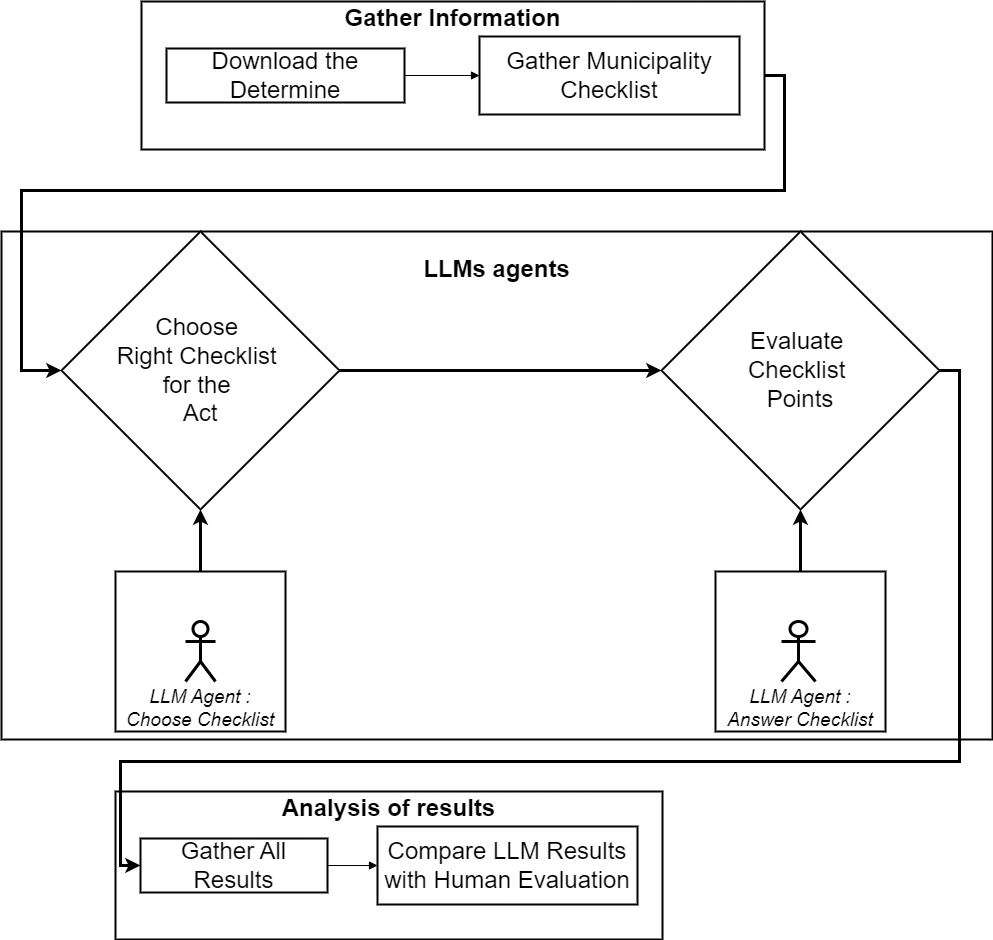
\includegraphics[width=10cm]{Graphs/0.Workflow.png}
\end{figure}


\section{Tools and Performance Metrics}
Several tools and performance metrics were used throughout the study:

\begin{itemize}
    \item \textbf{Software Tools:}
    \begin{itemize}
        \item Python for text extraction, prompt generation, and response processing.
        \item Regular expressions for cleaning and standardizing text outputs.
        \item OpenAI's API for accessing the LLM.
        \item Hugginface Transformers Library to load and use locally llama models
        \item CSV and JSON file handling for managing checklists and responses.
    \end{itemize}
    \item \textbf{Performance Metrics:}
    \begin{itemize}
        \item \textbf{Accuracy:} The degree to which the LLM's responses match the human-evaluated answers.
        \item \textbf{Consistency:} Variability in outputs with changes in the model's temperature and other parameters.
        \item \textbf{Efficiency:} Processing time and resource usage for automating the evaluation process.
        \item \textbf{Error Rate:} Frequency and nature of errors encountered during response extraction and analysis.
    \end{itemize}
\end{itemize}


\section{Data Preprocessing}
The preprocessing stage involved:

\begin{itemize}
    \item \textbf{Conversion of Checklists:}
 The checklists were transformed into a JSON format, segmenting each point into individual queries.
    \item \textbf{Text Extraction from PDFs:}
 Municipal determination documents were downloaded in PDF format and converted into plain text using Python scripts. This ensured that the text was in a consistent format for further analysis.
\end{itemize}
 

\section{Integration of the LLM}
Integration of the LLM into the workflow was implemented via a Python-based pipeline:

\begin{itemize}
    \item \textbf{Template-Based Querying:}
 A prompt template was developed to structure queries for the LLM. For each determination, the corresponding checklist was identified, and each point was queried individually using the template.
    \item \textbf{Automated Query Execution:}
 A Python program was created to loop over each document and checklist point, sending the prompt to the LLM and capturing the responses. The process is parameterized by:
    \begin{itemize}
        \item Model type (e.g., “gpt-4o-mini” vs. a larger model)
        \item Temperature settings (e.g., 0.0, 0.01, 0.5, 1.0) to assess consistency and output quality.
    \end{itemize}
    \item \textbf{Output Processing:}
 The raw outputs from the LLM, which are often lengthy, are parsed using regular expressions to extract standardized responses (SI/NO/NON PERTINENTE). The results for each document are compiled into a CSV file for further analysis.
\end{itemize}


\section{Workflow Diagram}
A workflow diagram (to be included as Figure X) summarizes the entire process:
\begin{enumerate}
    \item \textbf{Data Collection:} Download PDFs and extract text.
    \item \textbf{Checklist Selection:} Match documents with their corresponding checklists.
    \item \textbf{Prompt Generation:} Convert checklists into JSON and generate prompts.
    \item \textbf{LLM Querying:} Send prompts to the LLM and receive responses.
    \item \textbf{Response Extraction:} Use regex to parse and standardize responses.
    \item \textbf{Data Analysis:} Compare LLM results with manually compiled checklists.
\end{enumerate}
 

\section{Implementation Challenges}
During implementation, several challenges were encountered:

\begin{itemize}
    \item \textbf{Text Extraction Issues:}
 Converting PDFs to clean text sometimes resulted in formatting problems or loss of information.
    \item \textbf{Prompt Engineering:}
 Designing prompts that reliably guided the LLM was iterative; adjustments were made to ensure clarity and precision in the responses.
    \item \textbf{Regex Limitations:}
 Extracting the standardized SI/NO/NON PERTINENTE responses from long texts required robust regular expressions, which sometimes needed fine-tuning to accommodate unexpected output variations.
    \item \textbf{Model Variability:}
 Different temperature settings and model sizes influenced the consistency of outputs, necessitating multiple pilot tests.
\end{itemize}
 


\section{Pilot Tests}
Before finalizing the experimental setup, several pilot tests were conducted:

\begin{itemize}
    \item \textbf{Hyper-Parameter Tuning:}
 Experiments with various temperature settings helped determine the optimal balance between creativity and consistency in responses.
    \item \textbf{Validation:}
 Initial tests compared the LLM’s responses with a small set of manually evaluated documents to fine-tune the prompt design and extraction process.
    \item \textbf{Iterative Refinement:}
 Feedback from pilot tests led to improvements in the prompt template, regex patterns, and overall processing pipeline, ensuring that the final system was robust and reliable.
\end{itemize}


% Include bibliography only when compiling this subfile independently
\ifSubfilesClassLoaded{
    \bibliographystyle{sapthesis}
    \bibliography{Tesi}
}{}

\end{document}